\documentclass[10pt]{article}
\usepackage[utf8]{inputenc}
\usepackage[T1]{fontenc}
\usepackage{amsmath}
\usepackage{amsfonts}
\usepackage{amssymb}
\usepackage[version=4]{mhchem}
\usepackage{stmaryrd}
\usepackage{graphicx}
\usepackage[export]{adjustbox}
\graphicspath{ {./images/} }

\begin{document}
I cannot post the question or answer key for question 10 because it was derived from a secure AP Question. If you would like to review the key, you can come to FLEX or ask me during class.

\begin{enumerate}
  \item Given $f(x)=-2 \sin \left(\frac{\pi}{3} x-2\right)+4$, indicate each of the following (1 point each)
\end{enumerate}

\begin{center}
\begin{tabular}{|l|l|}
\hline
Domain: & Range: \\
\hline
Period: & Amplitude: \\
\hline
Coordinates of Relative Maxima: & x-intercept(s) \\
\hline
\end{tabular}
\end{center}

\begin{enumerate}
  \setcounter{enumi}{1}
  \item Graph the function $\boldsymbol{f}(\boldsymbol{x})=-\frac{1}{2} \cos \left(\frac{\boldsymbol{x}}{2}+\frac{\boldsymbol{\pi}}{2}\right)-2$. Show at least one period (4 points)\\
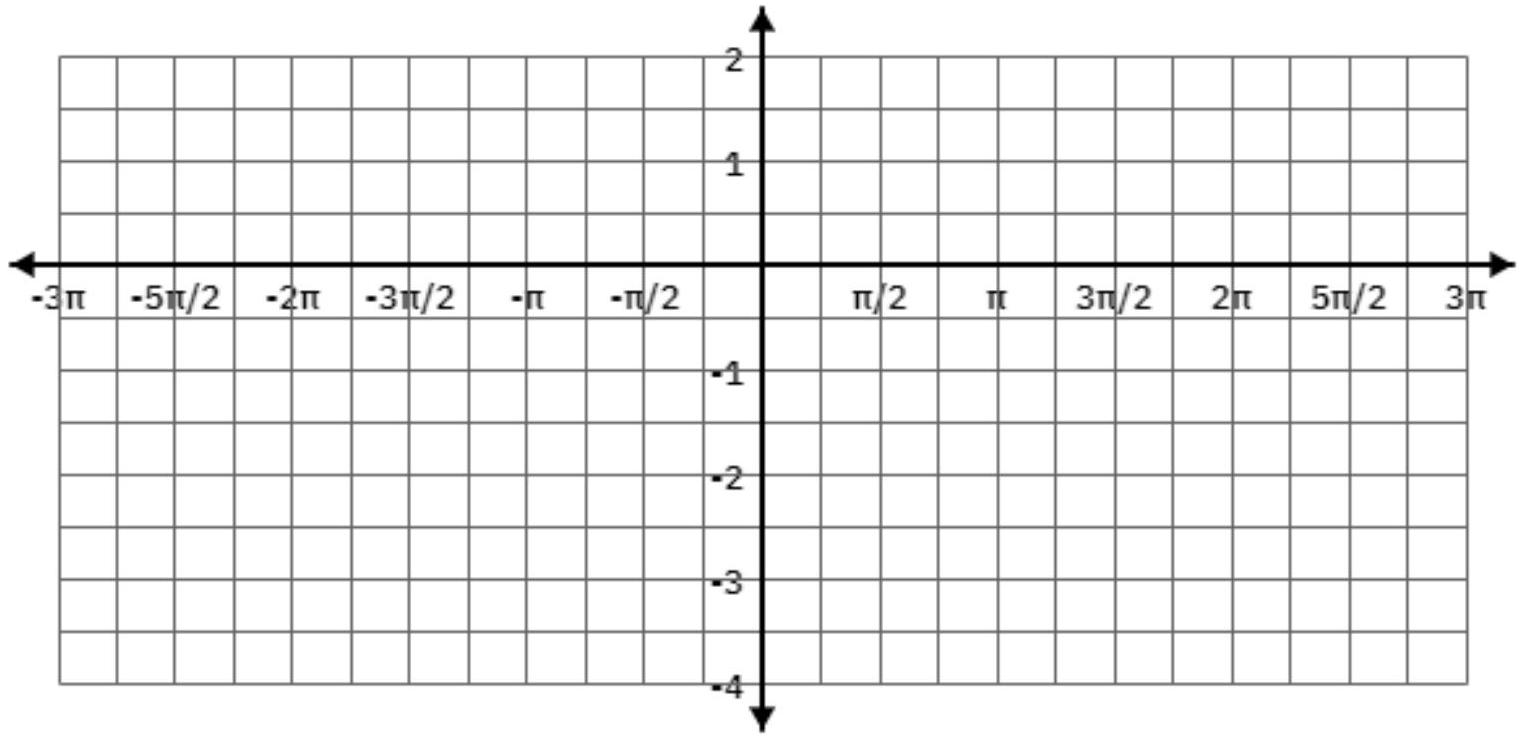
\includegraphics[max width=\textwidth, alt={}, center]{8853423f-17d5-40f7-87fd-f8886da86619-02_742_1525_941_201}
  \item Graph the function $\boldsymbol{f}(\boldsymbol{x})=-2 \csc (\boldsymbol{\pi} \boldsymbol{x}-\mathbf{2} \boldsymbol{\pi})$ - 3. Show at least one period (4 points)\\
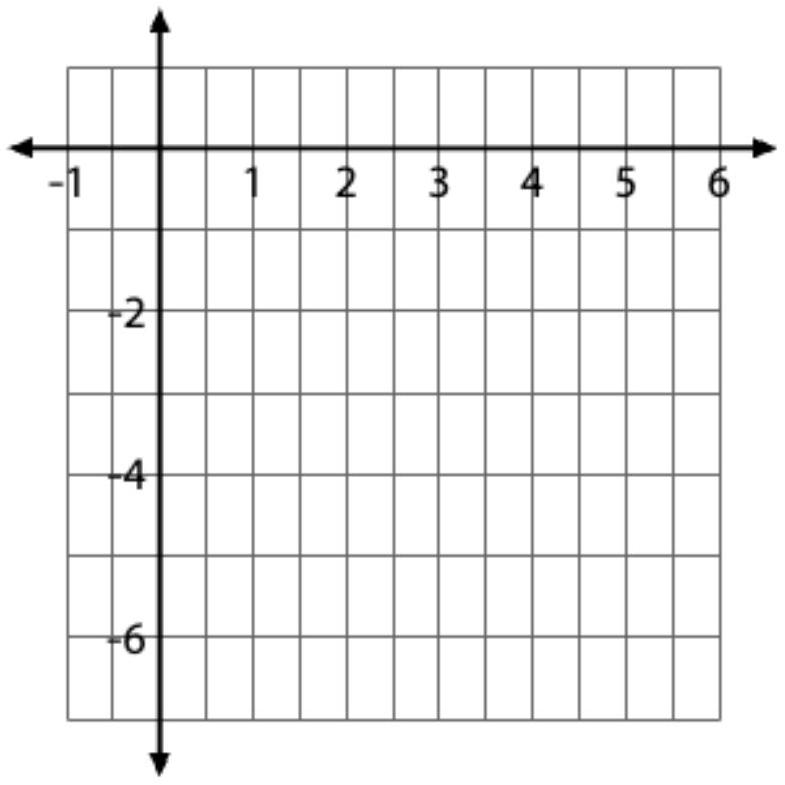
\includegraphics[max width=\textwidth, alt={}, center]{8853423f-17d5-40f7-87fd-f8886da86619-02_785_785_1873_343}
  \item A period of the function $p(x)=-3 \cot \left(\frac{\pi x}{7}-1\right)+3$ is shown below. If $B$ has coordinates $(h, k)$ and $0 \leq h \leq 7$, find the values requested below (1 point per item)\\
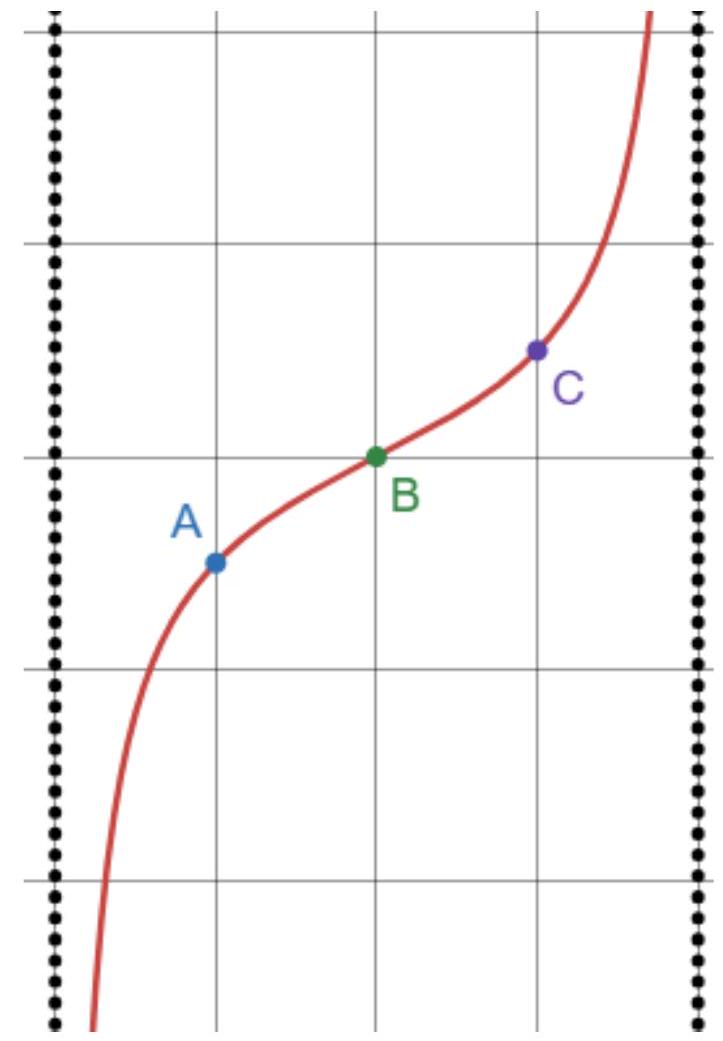
\includegraphics[max width=\textwidth, alt={}, center]{8853423f-17d5-40f7-87fd-f8886da86619-03_1041_723_313_64}
\end{enumerate}

Period of $p(x)$ : $\_\_\_\_$\\
All vertical asymptotes of $p(x)$ : $\_\_\_\_$\\
All Points of Inflection: $\_\_\_\_$\\
Coordinates of A: $\_\_\_\_$\\
Coordinates of B: $\_\_\_\_$\\
Coordinates of C: $\_\_\_\_$\\
5. Given $f(x)=-2 \sec \left(4 x-\frac{\pi}{11}\right)+8$, indicate each of the following (1 point each)

\begin{center}
\begin{tabular}{|l|l|}
\hline
Domain: & Range: \\
\hline
Period: & Amplitude: \\
\hline
State 4 different Vertical Asymptote(s) of $f(x)$ : & State the coordinates of all relative minima: \\
\hline
\end{tabular}
\end{center}

\begin{enumerate}
  \setcounter{enumi}{5}
  \item How many times does $\cos (600 x)=-\frac{1}{3}$ on the interval $\left(0, \frac{\pi}{6}\right]$ ( 1 point)?
\end{enumerate}

\begin{center}
\begin{tabular}{|l|l|l|}
\hline
\multicolumn{3}{|l|}{7. State the domain and range of each function shown below. (1 point per row)} \\
\hline
$f(x)$ & Domain & Range \\
\hline
$\operatorname{arcsec}(x)$ &  &  \\
\hline
$\arccos (x)$ &  &  \\
\hline
$\arctan (x)$ &  &  \\
\hline
\multicolumn{3}{|l|}{8. Evaluate each statement below. If no real value exists, write undefined. Show the work that leads to your answer. If you state that the expression is undefined, explain your reasoning. (2 points each)} \\
\hline
$\sin \left(-2 \arccos \left(-\frac{1}{2}\right)\right)$ &  & $\tan (\operatorname{arccsc}(2))$ \\
\hline
$\cos \left(\arcsin \left(\frac{\pi}{2}\right)\right)$ &  & $\cot \left(\operatorname{arcsec}\left(\frac{6}{5}\right)\right)$ \\
\hline
\multicolumn{3}{|l|}{9. The expression $\tan \left(\arccos \left(-\frac{13}{5}\right)\right)$ has no real value. However, it does have a complex value. Find the complex value of $\tan \left(\arccos \left(-\frac{13}{5}\right)\right)$. (2 points)} \\
\hline
\end{tabular}
\end{center}

\begin{enumerate}
  \item Given $f(x)=-3 \cos \left(\frac{\pi}{3} x-5\right)+4$, indicate each of the following (1 point each)
\end{enumerate}

\begin{center}
\begin{tabular}{|l|l|}
\hline
Domain: & Range: \\
\hline
Period: & Amplitude: \\
\hline
Coordinates of Relative Minima: & x-intercept(s) \\
\hline
\end{tabular}
\end{center}

\begin{enumerate}
  \setcounter{enumi}{1}
  \item Graph the function $\boldsymbol{f}(\boldsymbol{x})=-2 \sin \left(\frac{\boldsymbol{x}}{\mathbf{2}}+\frac{\boldsymbol{\pi}}{\mathbf{4}}\right)-\mathbf{2}$. Show at least one period (4 points)\\
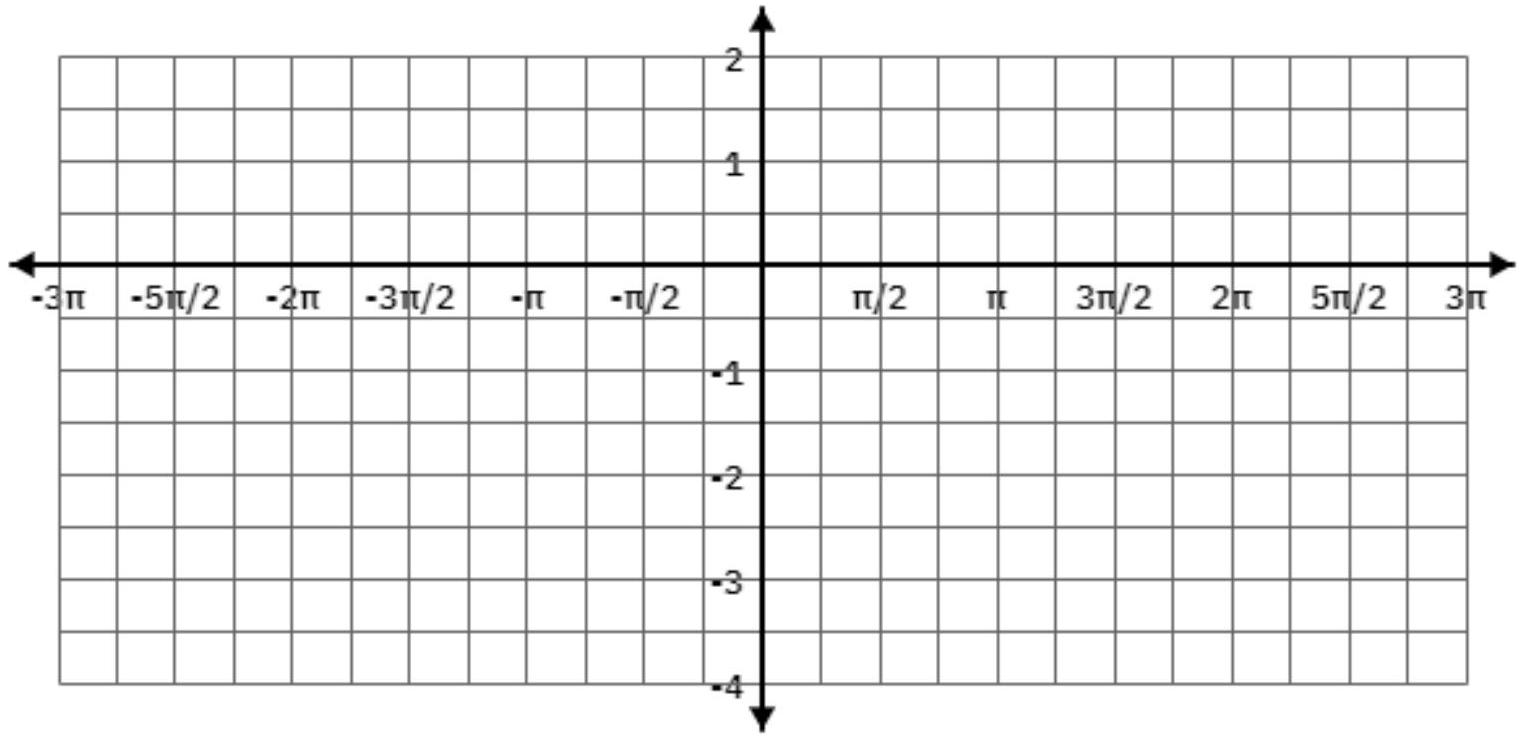
\includegraphics[max width=\textwidth, alt={}, center]{8853423f-17d5-40f7-87fd-f8886da86619-05_742_1525_941_201}
  \item Graph the function $\boldsymbol{f}(\boldsymbol{x})=2 \sec \left(\frac{\boldsymbol{\pi}}{2} \boldsymbol{x}-\boldsymbol{\pi}\right)$ - 3. Show at least one period (4 points)\\
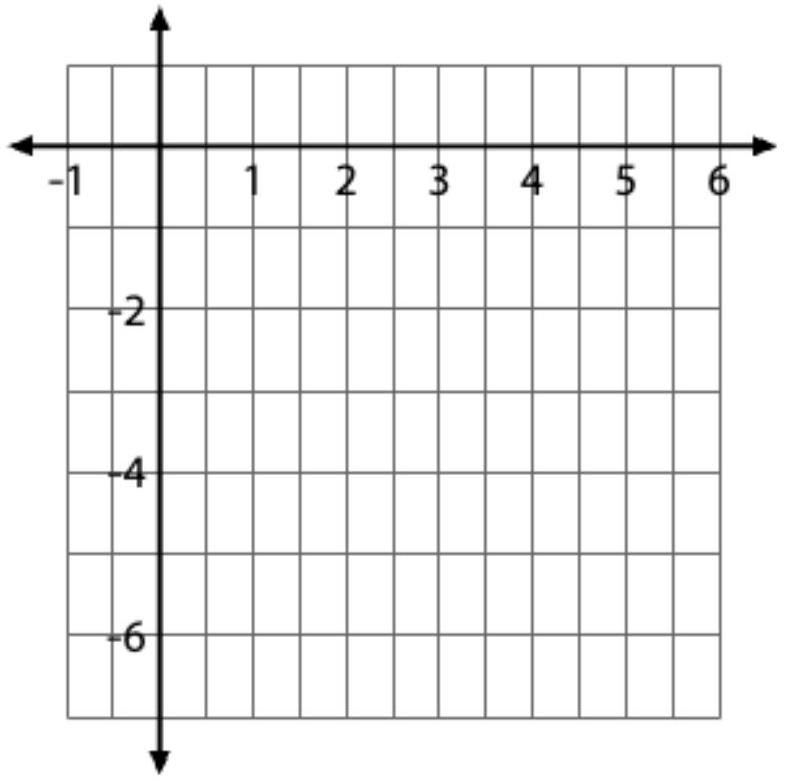
\includegraphics[max width=\textwidth, alt={}, center]{8853423f-17d5-40f7-87fd-f8886da86619-05_781_785_1875_343}
  \item A period of the function $p(x)=-6 \cot \left(\frac{\pi x}{3}-5\right)+3$ is shown below. If $B$ has coordinates $(h, k)$ and $0 \leq h \leq 3$, find the values requested below (1 point per item)\\
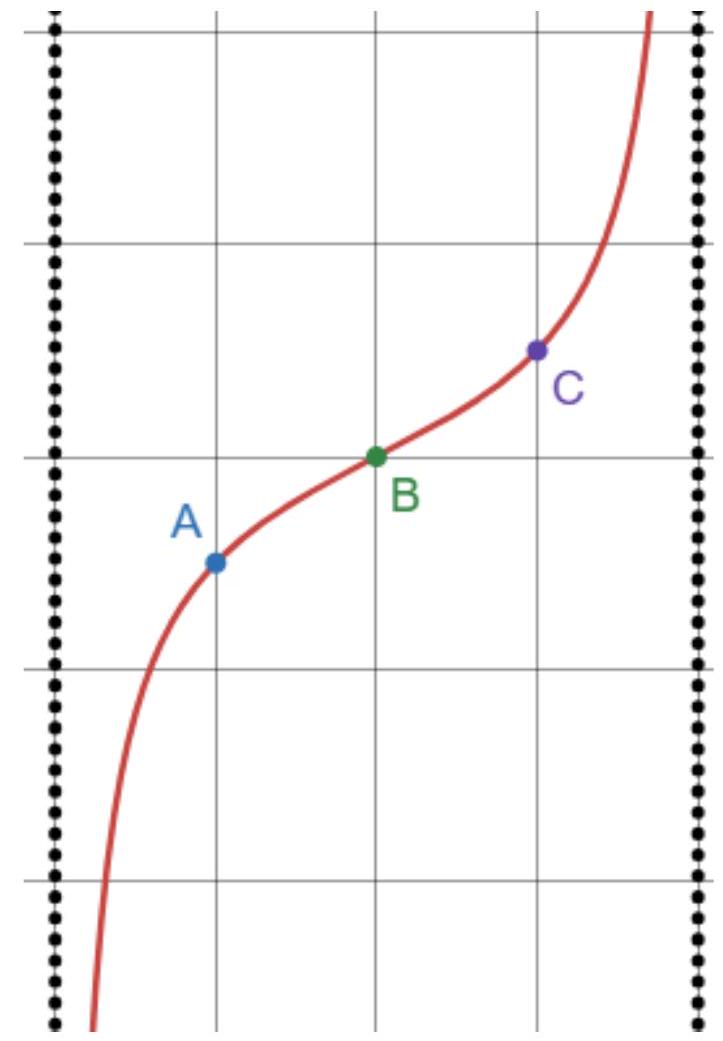
\includegraphics[max width=\textwidth, alt={}, center]{8853423f-17d5-40f7-87fd-f8886da86619-06_1041_723_313_64}
\end{enumerate}

Period of $p(x)$ : $\_\_\_\_$\\
All vertical asymptotes of $p(x)$ : $\_\_\_\_$\\
All Points of Inflection: $\_\_\_\_$\\
Coordinates of A: $\_\_\_\_$\\
Coordinates of B: $\_\_\_\_$\\
Coordinates of C: $\_\_\_\_$\\
5. Given $f(x)=-2 \sec \left(7 x-\frac{\pi}{3}\right)+18$, indicate each of the following (1 point each)

\begin{center}
\begin{tabular}{|l|l|}
\hline
Domain: & Range: \\
\hline
Period: & Amplitude: \\
\hline
State 4 different Vertical Asymptote(s) of $f(x)$ : & State the coordinates of all relative minima: \\
\hline
\end{tabular}
\end{center}

\begin{enumerate}
  \setcounter{enumi}{5}
  \item How many times does $\sin (800 x)=\frac{1}{6}$ on the interval $\left(0, \frac{\pi}{4}\right]$ ( 1 point)?
\end{enumerate}

\begin{center}
\begin{tabular}{|l|l|l|}
\hline
\multicolumn{3}{|l|}{7. State the domain and range of each function shown below. (1 point per row)} \\
\hline
$f(x)$ & Domain & Range \\
\hline
$\operatorname{arcsec}(x)$ &  &  \\
\hline
$\arcsin (x)$ &  &  \\
\hline
$\arctan (x)$ &  &  \\
\hline
\multicolumn{3}{|l|}{8. Evaluate each statement below. If no real value exists, write undefined. Show the work that leads to your answer. If you state that the expression is undefined, explain your reasoning. (2 points each)} \\
\hline
$\cos \left(-2 \arcsin \left(-\frac{1}{2}\right)\right)$ &  & $\cot (\operatorname{arcsec}(2))$ \\
\hline
$\cos \left(\arcsin \left(\frac{\pi}{3}\right)\right)$ &  & $\cot \left(\operatorname{arcsec}\left(-\frac{7}{4}\right)\right)$ \\
\hline
\multicolumn{3}{|l|}{9. The expression $\cot \left(\arccos \left(-\frac{13}{12}\right)\right)$ has no real value. However, it does have a complex value. Find the complex value of $\cot \left(\arccos \left(-\frac{13}{12}\right)\right)$. (2 points)} \\
\hline
\end{tabular}
\end{center}

\begin{enumerate}
  \item Given $f(x)=-2 \sin \left(\frac{\pi}{6} x+3\right)-34$, indicate each of the following (1 point each)
\end{enumerate}

Domain:

Period:

Coordinates of Relative Maxima:

Range:

Amplitude:\\
x-intercept(s)\\
2. Graph the function $\boldsymbol{f}(\boldsymbol{x})=-\frac{1}{2} \cos \left(\frac{\boldsymbol{x}}{2}-\frac{\mathbf{3} \boldsymbol{\pi}}{2}\right)-\mathbf{2}$. Show at least one period (4 points)\\
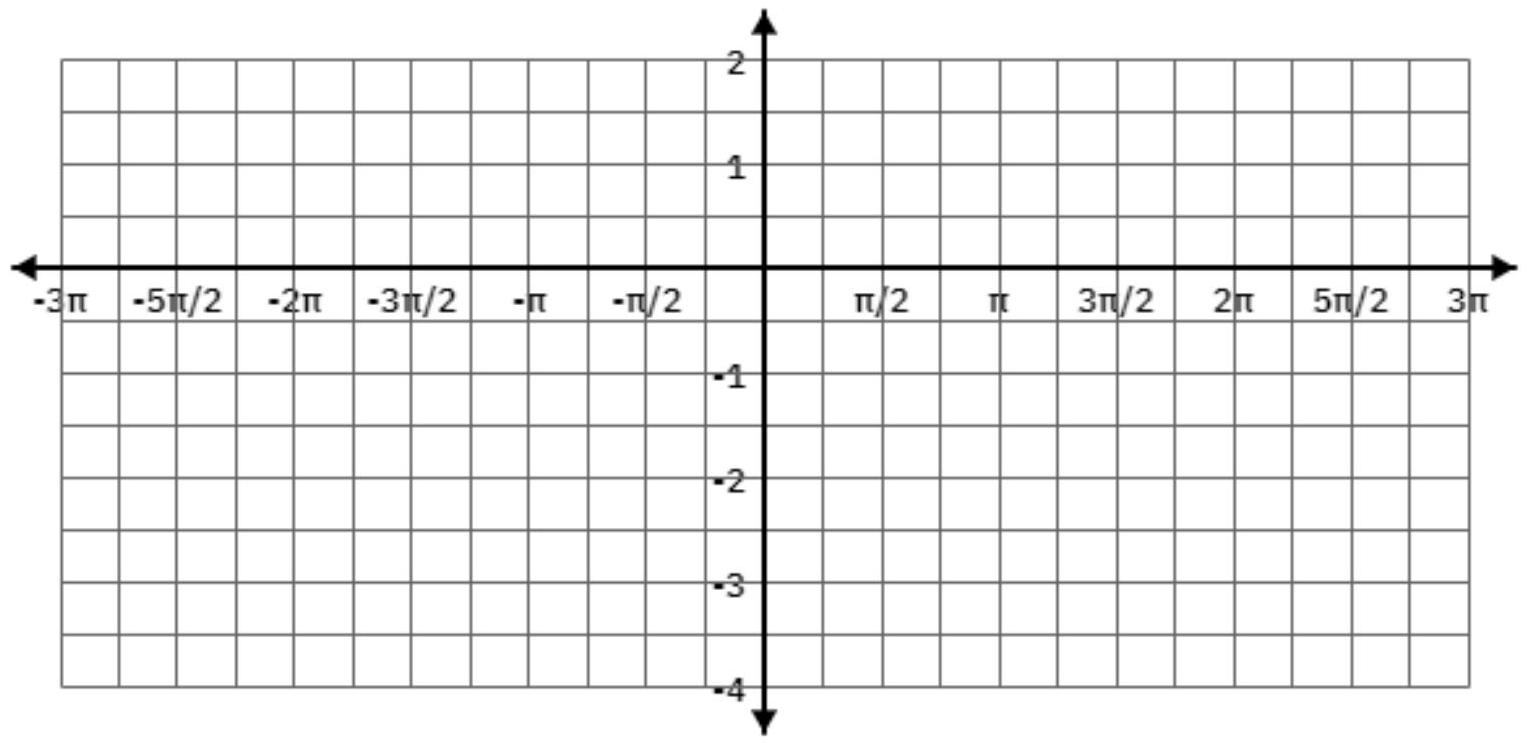
\includegraphics[max width=\textwidth, alt={}, center]{8853423f-17d5-40f7-87fd-f8886da86619-08_745_1527_938_199}\\
3. Graph the function $\boldsymbol{f}(\boldsymbol{x})=-2 \sec (\boldsymbol{\pi} \boldsymbol{x}-\mathbf{3} \boldsymbol{\pi})$ - 3. Show at least one period (4 points)\\
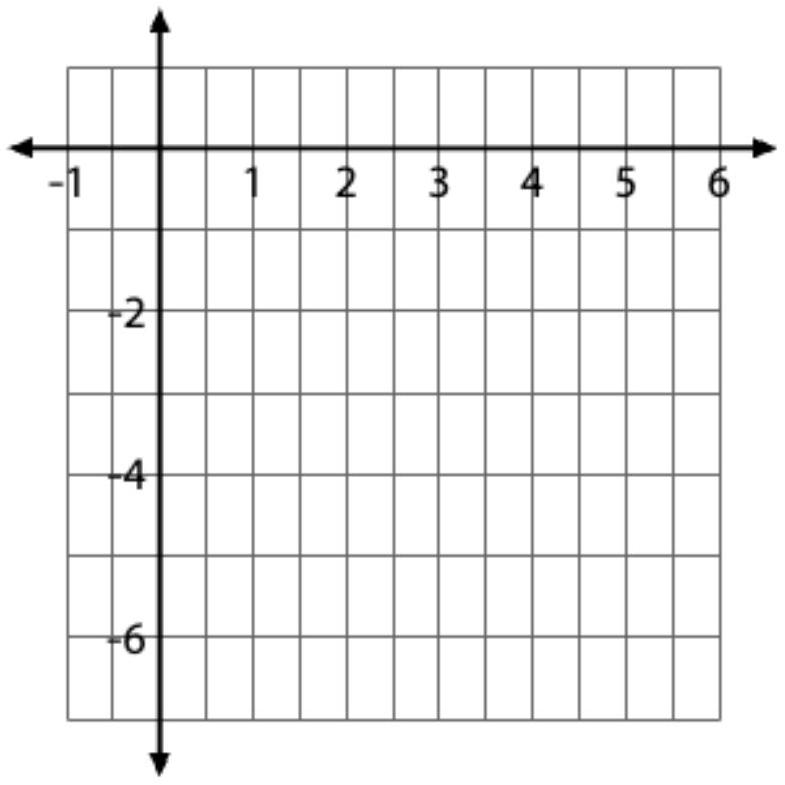
\includegraphics[max width=\textwidth, alt={}, center]{8853423f-17d5-40f7-87fd-f8886da86619-08_785_785_1873_343}\\
4. A period of the function $p(x)=7 \tan \left(\frac{\pi x}{6}-5\right)-23$ is shown below. If $B$ has coordinates $(h, k)$ and $0 \leq h \leq 6$, find the values requested below (1 point per item)\\
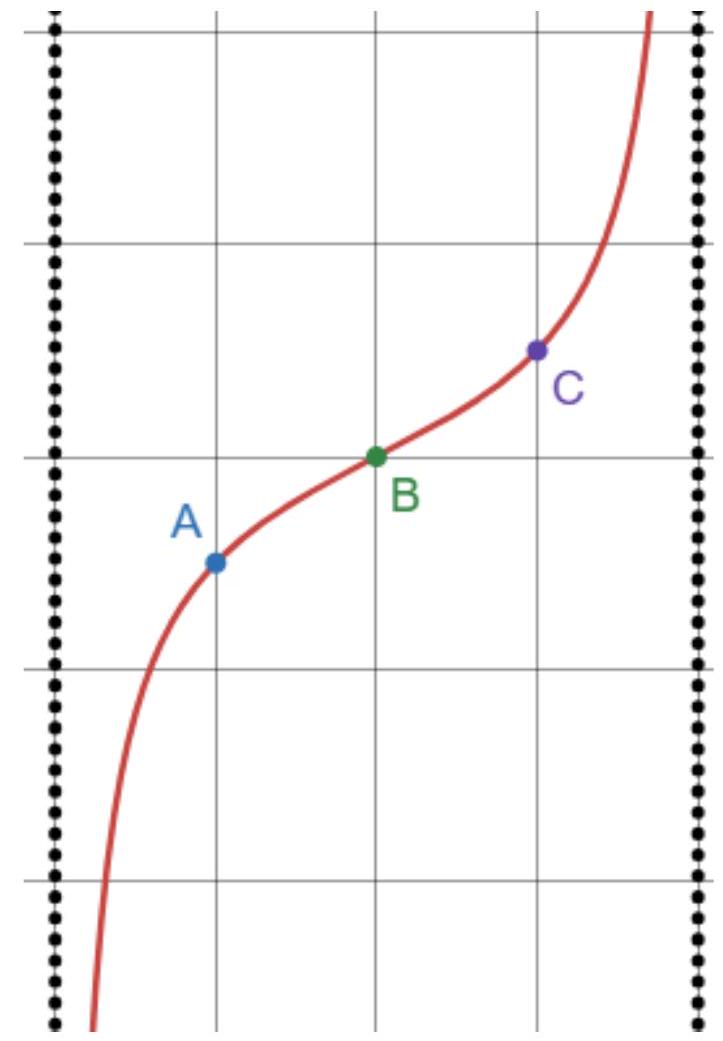
\includegraphics[max width=\textwidth, alt={}, center]{8853423f-17d5-40f7-87fd-f8886da86619-09_1041_723_313_64}

Period of $p(x)$ : $\_\_\_\_$\\
All vertical asymptotes of $p(x)$ : $\_\_\_\_$\\
All Points of Inflection: $\_\_\_\_$\\
Coordinates of A: $\_\_\_\_$\\
Coordinates of B: $\_\_\_\_$\\
Coordinates of C: $\_\_\_\_$\\
5. Given $f(x)=-5 \csc \left(3 x-\frac{2 \pi}{13}\right)+8$, indicate each of the following (1 point each)

Domain:\\
Range:

Period:\\
Amplitude:

State 4 different Vertical Asymptote(s) of $f(x)$ :\\
State the coordinates of all relative minima:\\
6. How many times does $\sin (1200 x)=\frac{1}{5}$ on the interval $\left(0, \frac{\pi}{3}\right]$ ( 1 point)?

\begin{center}
\begin{tabular}{|l|l|l|}
\hline
\multicolumn{3}{|l|}{7. State the domain and range of each function shown below. (1 point per row)} \\
\hline
$f(x)$ & Domain & Range \\
\hline
$\operatorname{arccsc}(x)$ &  &  \\
\hline
$\arccos (x)$ &  &  \\
\hline
$\operatorname{arccot}(x)$ &  &  \\
\hline
\multicolumn{3}{|c|}{8. Evaluate each statement below. If no real value exists, write undefined. Show the work that leads to your answer. If you state that the expression is undefined, explain your reasoning. (2 points each)} \\
\hline
$\sin \left(-2 \arccos \left(\frac{1}{2}\right)\right)$ &  & $\sec (\operatorname{arccsc}(2))$ \\
\hline
\multicolumn{2}{|c|}{$\cos \left(\arcsin \left(\frac{2 \pi}{3}\right)\right)$} & $\csc \left(\arctan \left(\frac{6}{5}\right)\right)$ \\
\hline
\multicolumn{3}{|l|}{9. The expression $\tan \left(\arccos \left(-\frac{5}{3}\right)\right)$ has no real value. However, it does have a complex value. Find the complex value of $\tan \left(\arccos \left(-\frac{5}{3}\right)\right)$. (2 points)} \\
\hline
\end{tabular}
\end{center}


\end{document}